% Created 2017-05-04 Thu 21:33
% Intended LaTeX compiler: pdflatex
\documentclass[journal=ancac3,manuscript=suppinfo,email=true]{achemso}
 \usepackage{minted}
 \usepackage{graphicx}
\usepackage{float}
\usepackage{xcolor}
\usepackage{amsmath}
\usepackage{fontspec}
\author{Tian Tian}
\affiliation{Institute for Chemical and Bioengineering, ETH Z{\"{u}}rich,  Vladimir Prelog Weg 1, CH-8093 Z{\"{u}}rich, Switzerland}
\author{Elton J. G. Santos}
\affiliation{School of Mathematics and Physics, Queen's University Belfast, United Kingdom}
\affiliation{School of Chemistry and Chemical Engineering, Queen's University Belfast, United Kingdom}
\author{Shangchao Lin}
\email{slin@eng.fsu.edu.}
\affiliation{Department of Mechanical Engineering, Materials Science and Engineering Program, FAMU-FSU College of Engineering, Florida State University, Tallahassee, Florida 32310, United States}
\author{Chih-Jen Shih}
\email{chih-jen.shih@chem.ethz.ch}
\affiliation{Institute for Chemical and Bioengineering, ETH Z{\"{u}}rich,  Vladimir Prelog Weg 1, CH-8093 Z{\"{u}}rich, Switzerland}
\date{}
\title{Wettability of Doped Two-Dimensional Materials}
\begin{document}

\newpage{}
\section{Figures}
\label{sec:org176b821}
\subsection{Dipole Orientation Profiles of MD Simulations}
\label{sec:org3abd37b}
\begin{figure}[htbp]
\centering
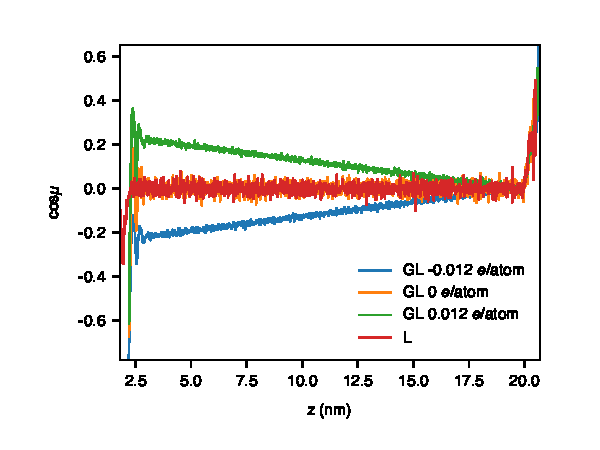
\includegraphics[width=0.85\linewidth]{../img/SI-dipole-profile.pdf}
\caption{\label{fig-SI-dipole}
Dipole orientation \(\cos \mu\) as a function of \(z\) in MD simulations of different systems (L, and GL with varied graphene doping densities). The orientation at the water-vacuum interface (\$z\$=20 nm) is invariable in all cases, indicating a minimal effect of the long range Coulombic interaction on the selected interface.}
\end{figure}

\newpage{}
\subsection{Hydrogen Bond Profiles of MD Simulations}
\label{sec:orge06c9b9}

\begin{figure}[htbp]
\centering
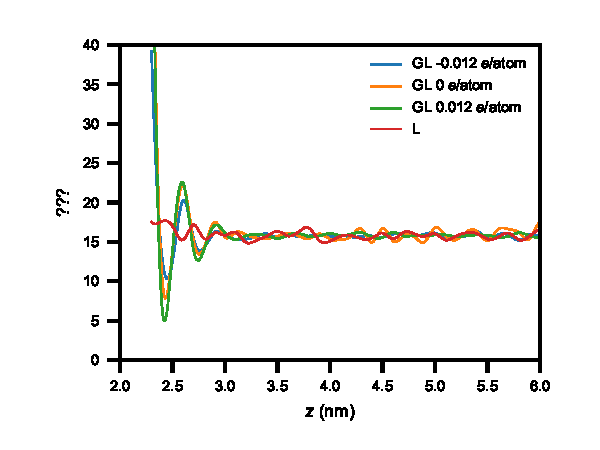
\includegraphics[width=0.85\linewidth]{../img/hydrogen-bond.pdf}
\caption{\label{fig-H-bond}
Hydrogen bond strength as a function of \(z\) in MD simulations of various conditions (L, GL with graphene doping densities of -0.012, 0 and 0.012 \$e\$/atom).}
\end{figure}

\begin{center}
\fbox{
\begin{minipage}[c]{.8\linewidth}
\textbf{\textsf{\textsc{TODO}}} Ask Prof. Lin for unit and explanation of H-Bond result

\end{minipage}
}
\end{center}
\newpage{}
\subsection{Fitting of the \(\Delta \Phi\) - \(\sigma_{\mathrm{2D}}\) Data in MD Simulations}
\label{sec:orgb2e4751}
\begin{figure}[htbp]
\centering
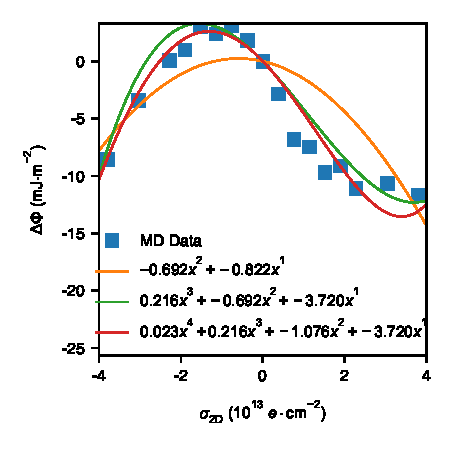
\includegraphics[width=0.85\linewidth]{../img/e-Phi-fitting.pdf}
\caption{\label{fig-SI-fitting}
Fitting of \(\Delta \Phi\) - \(\sigma_{\mathrm{2D}}\) data from MD simulations with different polynomial functions. The 3rd degree polynomial function is chosen as the best fitting model.}
\end{figure}
\end{document}